\documentclass[11pt]{article}
\usepackage[T1]{fontenc}
\usepackage{mathpazo}
\renewcommand{\ttdefault}{pcr}
\usepackage[margin=0.9in]{geometry}
\usepackage{booktabs,array,multirow,graphicx,float,caption,enumitem,xcolor,listings,fancyhdr,microtype}
\usepackage[hidelinks]{hyperref}
\setlength{\tabcolsep}{4pt}
\newcommand{\tTwoWoneCycles}{22}
\newcommand{\tTwoWfourCycles}{10}
\newcommand{\tTwoWfourCdbOne}{19}
\newcommand{\tOneWone}{57}
\newcommand{\tOneWfour}{51}
\newcommand{\tThreeWone}{31}
\newcommand{\tThreeWfour}{26}
\newcommand{\tSevenWone}{36}
\newcommand{\tSevenWtwo}{33}
\newcommand{\tEightWone}{47}
\newcommand{\tEightWtwo}{46}
\newcommand{\tSixAll}{28}
\newcommand{\tFiveWtwoSquashed}{29}


\definecolor{codebg}{HTML}{F6F5F1}
\lstset{basicstyle=\ttfamily\footnotesize,backgroundcolor=\color{codebg},frame=none,
        columns=fullflexible,keepspaces=true,showstringspaces=false,xleftmargin=4pt,aboveskip=6pt}
\captionsetup{font=small,labelfont=bf}
\setlist{itemsep=2pt,topsep=4pt}
\pagestyle{fancy}\fancyhf{}
\lhead{\small Computer Architecture}\rhead{\small Programming Assignment: Tomasulo (multi-issue)}
\cfoot{\small\thepage}
\renewcommand{\headrulewidth}{0.4pt}

\title{\textbf{Programming Assignment: Tomasulo Algorithm}\\[2pt]
\large Adding in-order multi-issue (1--4 instructions per cycle) to the Tomasulo simulator}
\author{Ilan Lipsky}
\date{}

\begin{document}
\maketitle
\thispagestyle{fancy}

\section{Overview}
The assignment starts from an existing Python simulator of Tomasulo's algorithm with a reorder
buffer (ROB), register alias tables (RAT) and a load/store queue (LSQ), and asks for support for
issuing $W = 1$--$4$ instructions per cycle, in program order, with the issue width given in the
input file. In summary, I:

\begin{itemize}
  \item added \textbf{in-order multi-issue} (issue width 1--4, default 1), a \textbf{multi-commit}
        stage (commit width, defaults to the issue width) and a configurable number of
        \textbf{CDBs} (default 1, as in the handout);
  \item implemented the \textbf{branch unit} the handout specifies but the original code lacked:
        8-entry BTB indexed by the 3 low bits of the PC word address, a 1-bit predictor per
        entry, prediction in ISSUE, resolution at the end of EX, and \textbf{misprediction
        recovery} (RAT recovery, RS/LSQ/FU/CDB-queue clean-up, ROB squash, correct fetch at
        cycle $n{+}2$). Without it, multi-issue past a branch is impossible;
  \item made the hardware \textbf{fully parameterizable from the input file} (RS counts, EX/MEM
        latencies, \# of FUs, ROB size, issue/commit/CDB width, initial registers and memory),
        added \texttt{Beq} and \texttt{Sub}/\texttt{Sub.d}, and print the required final
        \textbf{register and non-zero memory} values;
  \item built a \textbf{verification harness}: a sequential golden model, timing-invariant
        checks, 9 directed test benches $\times$ 4 issue widths $\times$ 2 CDB settings, and
        20{,}000 random differential runs. All pass.
\end{itemize}

\section{Starting point}
The provided code (\texttt{code/*.py}, Qing, 2017) simulates single-issue Tomasulo with
speculation-free branch handling. Reading and running it showed the following limitations that
shaped the work:
\begin{itemize}
  \item \textbf{One instruction per cycle} everywhere: one issue, one CDB latch, at most one
        commit (plus a special case for a store followed by one more instruction).
  \item \textbf{No branch prediction}: at every \texttt{Bne} fetch is switched off
        (\texttt{PC.valid = 0}) until the branch resolves. \texttt{Beq} is not supported, and the
        branch offset is treated as a \emph{byte} offset (\texttt{offset/4}) while the ISA defines
        \texttt{PC+4+offset<<2}.
  \item \textbf{Hard-coded configuration}: RS sizes, latencies, ROB size and initial values are
        constants in \texttt{main.py}; \texttt{test\_case.txt} is never read. Registers and memory
        are not printed, and branches are printed with an empty commit column.
  \item Records are \texttt{namedtuple} \emph{classes} whose class attributes are mutated, and
        \texttt{mem.py} has latent bugs (\texttt{if (check\_if\_sd\_committable):} tests the
        function object instead of calling it; that function reads a non-existent field
        \texttt{ldsd\_tag}; the load-dispatch test checks \texttt{ld\_sd\_queue[0].data} instead
        of the entry being considered).
\end{itemize}
Since nearly every function had to accept $W$ instructions per cycle and cope with squashed
speculative state, I kept the original module structure (\texttt{init}, \texttt{issue},
\texttt{exe}, \texttt{mem}, \texttt{wb}, \texttt{commit}, \texttt{print\_status}, \texttt{main}),
but rewrote the bodies around small explicit record classes.

\section{What was added to the code}
\begin{table}[H]\centering\small
\begin{tabular}{@{}>{\ttfamily}l p{0.70\textwidth}@{}}\toprule
\normalfont File & Changes \\\midrule
init.py & Input-file parser (hardware table, \texttt{Issue width}, \texttt{Commit width},
  \texttt{CDB width}, \texttt{ROB entries}, registers, memory, program; case-insensitive, commas
  optional); record classes \texttt{ROBEntry}, \texttt{RSEntry}, \texttt{LSQEntry}, \texttt{FU};
  \texttt{Machine} state; \texttt{squash\_after()} misprediction recovery. \\
issue.py & Issue up to $W$ instructions per cycle in program order; stop at the first structural
  hazard (ROB, RS or LSQ full) and after a predicted-taken branch; BTB lookup for branches; no
  issue during misprediction recovery. \\
predictor.py & \emph{New.} 8-entry BTB (index = word address \texttt{\&\,7}, tag = PC) with
  target and 1-bit taken/not-taken state; miss $\Rightarrow$ predict not-taken. \\
exe.py & Several FUs per class; pipelined FP adder/multiplier (one new op per cycle each),
  unpipelined integer and address adders; oldest-ready-first selection; \texttt{Beq}/\texttt{Bne}
  resolution, BTB update and squash. \\
mem.py & Conservative disambiguation, store-to-load forwarding (1 cycle), single-ported
  non-pipelined memory, LSQ entry freed when a load gets its value. \\
wb.py & Up to \texttt{CDB width} broadcasts per cycle, oldest instruction first. \\
commit.py & Up to \texttt{Commit width} in-order commits per cycle; stores write memory at commit
  and hold the single memory port; memory-fault reporting for committed instructions only. \\
print\_status.py & Required output: instruction status table, R0--R31, F0--F31, non-zero
  memory, plus a summary (cycles, IPC, mispredictions, squashed instructions). \\
main.py & Cycle loop, command-line options (\texttt{-w}, \texttt{--cdb}, \texttt{--commit},
  \texttt{-v} cycle trace, \texttt{--btb}). \\
tools/ & \emph{New.} Golden model, invariant checks, test runner, random fuzzer. \\
\bottomrule\end{tabular}
\caption{Summary of the changes by file.}
\end{table}

\subsection{Multi-issue (ISSUE stage)}
Each cycle the issue stage fetches from the PC and issues up to $W$ instructions \emph{in order}.
For each one it needs a free ROB entry and a free entry in its reservation station (integer adder
for \texttt{Add}, \texttt{Addi}, \texttt{Sub}, \texttt{Beq} and \texttt{Bne}; FP adder, FP multiplier) or in the LSQ (\texttt{Ld/Sd}). The
first instruction that cannot get its entries stops issue for the cycle, so a younger instruction
never overtakes it. Sources are read through the RAT \emph{before} the destination is renamed, so
same-cycle dependences inside an issue group (e.g.\ \texttt{Addi R1,R1,8} followed by
\texttt{Ld F1,0(R1)}) are renamed correctly: the second instruction waits on the first one's ROB
tag. A branch is predicted with the BTB at issue. If it is predicted taken, the fetch group ends
and the target is fetched next cycle; otherwise issue continues down the fall-through path in the
same cycle.

\subsection{Wider back end}
Issuing $W$ instructions per cycle only helps if the rest of the machine keeps up, so the
back end is widened as well:
\begin{itemize}
  \item \textbf{Commit width} (default $=W$): up to that many ROB-head instructions retire per cycle.
  \item \textbf{CDB width} (default 1, the handout's ``one CDB''): number of results broadcast per
        cycle. Results waiting for a bus are picked oldest-first. Section~\ref{sec:results} reports
        both 1 CDB and $W$ CDBs, because with one bus the CDB becomes the bottleneck.
  \item \textbf{Multiple functional units} per class (the ``\# of FUs'' column), each choosing the
        oldest ready instruction from its reservation stations.
\end{itemize}

\subsection{Branch prediction and speculation}
Branches go to the integer-adder reservation stations and use the integer adder to compare. At
the end of EX (cycle $n$) the branch updates its BTB entry. If the actual next PC differs from the
predicted one, \texttt{squash\_after()} removes every younger instruction from the ROB, the
reservation stations (including their wait-for tags), the LSQ, the functional units and the CDB
queue. It then rebuilds the RAT from the surviving ROB entries. Cycle $n{+}1$ is the recovery
cycle, and fetch from the correct path starts in cycle $n{+}2$, as the handout requires (e.g.\
\texttt{test1}, $W{=}1$: the \texttt{Bne} resolves in cycle 10 and the next \texttt{Ld} issues in
cycle 12). Wrong-path instructions never touch architectural state, because registers are
written only at commit and stores write memory only at commit. A wrong-path load that faults (bad
address) is flagged and only reported if it commits.

\subsection{Load/store queue}
Loads and stores enter the LSQ in program order and compute their address on a dedicated
address adder. In MEM, a load waits while any older store address is still unknown
(conservative disambiguation, as in the original code). Otherwise it forwards from the nearest
older store with the same address in 1 cycle, once that store's data is available, or else
accesses the single-ported, non-pipelined memory for \texttt{Cycles in Mem} cycles. Stores are
dequeued at commit, when they write memory and occupy the port for \texttt{Cycles in Mem} cycles
(shown as their MEM interval). A store that commits in a cycle can still forward to a load in that
same cycle. I found this case through \texttt{test4}: before handling it, \texttt{test4} ran
\emph{slower} at $W{=}2$ (30 cycles) than at $W{=}1$ (27), because a store that committed earlier
under wider commit could no longer forward its value.

\section{Timing model}
\begin{table}[H]\centering\small
\begin{tabular}{@{}l p{0.72\textwidth}@{}}\toprule
Stage & Rule (cycle numbers as printed in the tables) \\\midrule
ISSUE & $\le W$ per cycle, in order; resources freed earlier in the same cycle may be reused. \\
EX & starts $\ge$ ISSUE$+1$ and $\ge$ (last operand's WB)$+1$; lasts \texttt{Cycles in EX}. \\
MEM (Ld) & starts $\ge$ EX end$+1$; \texttt{Cycles in Mem} cycles, or 1 cycle if forwarded. \\
WB & $\ge$ EX end$+1$ (ALU) or MEM end$+1$ (Ld); $\le$ \texttt{CDB width} per cycle. Stores and branches have no WB. \\
COMMIT & in order, $\le$ commit width per cycle; $\ge$ WB$+1$ (ALU, Ld), $\ge$ EX end$+1$
  (branch); a store commits once address and data are known and the memory port is free. \\
Mispredict & detected at EX end $n$; recovery in $n{+}1$; correct-path ISSUE from $n{+}2$. \\
\bottomrule\end{tabular}
\caption{Pipeline timing rules. Each cycle evaluates COMMIT, WB, MEM, EX, ISSUE; all hand-offs are
time-stamped so an instruction never passes two dependent stages in one cycle.}
\end{table}

\section{Verification}
Each run is checked automatically (\texttt{tools/checks.py}):
\begin{enumerate}
  \item \textbf{Functional}: final R0--R31, F0--F31 and all 256 memory cells must equal those of an
        independent sequential interpreter (\texttt{tools/reference.py}), and the committed
        instruction stream must equal the interpreter's dynamic trace (so no wrong-path
        instruction commits and none is lost).
  \item \textbf{Timing invariants}: in-order issue and commit; $\le W$ issued, $\le$ commit-width
        committed and $\le$ CDB-width broadcast per cycle; ISSUE $<$ EX $<$ (MEM) $<$ WB $<$
        COMMIT; correct EX/MEM lengths; every consumer starts EX after its producer's WB; stores
        commit after their data is broadcast; one memory access at a time.
\end{enumerate}
\texttt{tools/run\_tests.py} runs the 9 test benches at $W = 1..4$ with one CDB and with $W$ CDBs
(72 runs). \texttt{tools/fuzz.py} generates random programs (ALU ops, aliasing loads/stores, forward
branches, counted loops) on random machines (ROB 2--64, 1--4 RS, 1--2 FUs, varied latencies,
CDB 1--4) and runs each at all four widths. Two seeds, 5{,}000 programs and 20{,}000 runs, exercised
about 52{,}000 mispredictions, 96{,}000 squashed instructions and 15{,}000 forwards with
\textbf{0 failures}. To check that the checker itself catches errors, I injected bugs on purpose:
skipping RAT recovery deadlocks, broadcasting more than the CDB width trips the CDB invariant, and
forwarding before store data is ready fails both \texttt{test4} and the fuzzer.

\section{Test cases}
\begin{table}[H]\centering\small
\begin{tabular}{@{}l p{0.78\textwidth}@{}}\toprule
Test & Purpose \\\midrule
\texttt{test0} & Configuration from the handout (\texttt{Issue width = 2}). The handout's 3-line program loops forever (\texttt{R2}$\neq$\texttt{R3}), so a decrement of R2 was added: the loop runs twice, and both branches mispredict (cold BTB, then loop exit). \\
\texttt{test1} & The loop shipped with the original code: Ld/Mult/Ld/Add/Sd over 3 elements, with \texttt{Bne} offset $-8$ (words). Exercises speculation, LSQ capacity and memory. \\
\texttt{test2} & 16 independent int/FP instructions on 2 units of each type: best case for multi-issue. \\
\texttt{test3} & One RAW chain with WAR/WAW name dependences: width cannot help; renaming must be right. \\
\texttt{test4} & Store-to-load forwarding, a load stalled behind a store with unknown address, a load to a different address, two stores to the same address. \\
\texttt{test5} & Nested loops with \texttt{Beq}/\texttt{Bne} (3$\times$2 iterations), an unconditional \texttt{Beq R0,R0}, and wrong-path code that would corrupt R9/F9/memory if squashing failed. \\
\texttt{test6} & Structural hazards: 4-entry ROB, 1--2 RS per unit, unpipelined 2-cycle integer adder. \\
\texttt{test7}, \texttt{test8} & ``Test Case \#01/\#02'' from the sample report, for comparison. \\
\bottomrule\end{tabular}
\end{table}

\section{Results under different issue widths}\label{sec:results}
All runs below finish with the same, correct registers and memory at every width (Section~\ref{sec:final}).
Full outputs for every test, width and CDB setting are in \texttt{results/}.

\begin{table}[H]\centering\small
\begin{tabular}{@{}lr rrrr rrr r@{}}\toprule
& & \multicolumn{4}{c}{CDB width = 1} & \multicolumn{3}{c}{CDB width = W} & Best\\\cmidrule(lr){3-6}\cmidrule(lr){7-9}
Test & Instr. & W=1 & W=2 & W=3 & W=4 & W=2 & W=3 & W=4 & speedup\\\midrule
\texttt{test0} & 8 & 19 & 15 & 13 & 13 & 15 & 13 & 13 & 1.46$\times$\\
\texttt{test1} & 25 & 57 & 52 & 51 & 51 & 52 & 51 & 51 & 1.12$\times$\\
\texttt{test2} & 16 & 22 & 19 & 19 & 19 & 14 & 12 & 10 & 2.20$\times$\\
\texttt{test3} & 10 & 31 & 28 & 27 & 27 & 28 & 27 & 26 & 1.19$\times$\\
\texttt{test4} & 13 & 27 & 23 & 23 & 22 & 23 & 23 & 22 & 1.23$\times$\\
\texttt{test5} & 37 & 71 & 56 & 56 & 54 & 54 & 53 & 53 & 1.34$\times$\\
\texttt{test6} & 10 & 28 & 28 & 28 & 28 & 28 & 28 & 28 & 1.00$\times$\\
\texttt{test7} & 17 & 36 & 35 & 35 & 35 & 33 & 33 & 33 & 1.09$\times$\\
\texttt{test8} & 17 & 47 & 46 & 46 & 46 & 46 & 46 & 46 & 1.02$\times$\\
\bottomrule\end{tabular}

\caption{Total cycles. \emph{Best speedup} = cycles at $W{=}1$ / fewest cycles at any width and CDB setting.}
\end{table}
\begin{table}[H]\centering\small
\begin{tabular}{@{}l rrrr rrr r@{}}\toprule
& \multicolumn{4}{c}{CDB width = 1} & \multicolumn{3}{c}{CDB width = W} & Mispred. /\\\cmidrule(lr){2-5}\cmidrule(lr){6-8}
Test & W=1 & W=2 & W=3 & W=4 & W=2 & W=3 & W=4 & squashed (W=1)\\\midrule
\texttt{test0} & 0.42 & 0.53 & 0.62 & 0.62 & 0.53 & 0.62 & 0.62 & 2 / 2\\
\texttt{test1} & 0.44 & 0.48 & 0.49 & 0.49 & 0.48 & 0.49 & 0.49 & 2 / 1\\
\texttt{test2} & 0.73 & 0.84 & 0.84 & 0.84 & 1.14 & 1.33 & 1.60 & 0 / 0\\
\texttt{test3} & 0.32 & 0.36 & 0.37 & 0.37 & 0.36 & 0.37 & 0.38 & 0 / 0\\
\texttt{test4} & 0.48 & 0.57 & 0.57 & 0.59 & 0.57 & 0.57 & 0.59 & 0 / 0\\
\texttt{test5} & 0.52 & 0.66 & 0.66 & 0.69 & 0.69 & 0.70 & 0.70 & 8 / 14\\
\texttt{test6} & 0.36 & 0.36 & 0.36 & 0.36 & 0.36 & 0.36 & 0.36 & 0 / 0\\
\texttt{test7} & 0.47 & 0.49 & 0.49 & 0.49 & 0.52 & 0.52 & 0.52 & 0 / 0\\
\texttt{test8} & 0.36 & 0.37 & 0.37 & 0.37 & 0.37 & 0.37 & 0.37 & 0 / 0\\
\bottomrule\end{tabular}

\caption{IPC (committed instructions / cycles), and branch mispredictions / squashed instructions at $W{=}1$.}
\end{table}

\begin{figure}[H]\centering
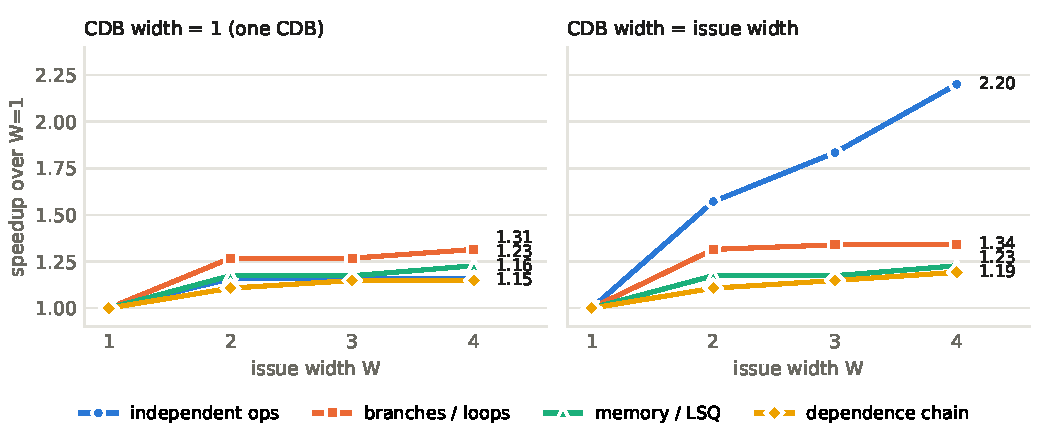
\includegraphics[width=\textwidth]{generated/speedup.pdf}
\caption{Speedup over single issue for four representative tests. Left: one CDB; right: one CDB per issue slot.}
\end{figure}

\paragraph{Discussion.} Multi-issue always helps or is neutral; no test gets slower as $W$ grows.
How much it helps depends on what limits the program:
\begin{itemize}
  \item \textbf{Independent instructions} (\texttt{test2}): \tTwoWoneCycles{} $\to$ \tTwoWfourCycles{}
        cycles at $W{=}4$ with 4 CDBs (IPC 0.73 $\to$ 1.60). With a single CDB the same machine stops
        at \tTwoWfourCdbOne{} cycles, because at most one result per cycle can be written back.
  \item \textbf{True dependences} (\texttt{test3}) and \textbf{long-latency chains} (\texttt{test1},
        \texttt{test7}, \texttt{test8}, which are dominated by 15--20 cycle multiplies feeding adds)
        gain only 2--19\%. Wider issue just fills the reservation stations earlier.
  \item \textbf{Branches} (\texttt{test0}, \texttt{test5}): each misprediction still costs the
        $n{+}2$ restart, but more instructions issue between restarts, so the gain is 31--46\%.
  \item \textbf{Structural limits} (\texttt{test6}): the 4-entry ROB caps the window, so all
        widths take \tSixAll{} cycles. Issue stalls in order whenever the ROB or an RS is full.
  \item \textbf{Sample-report cases}: at $W{=}1$, \texttt{test7} takes \tSevenWone{} cycles
        (sample report: 36), and at $W{=}2..4$ with $W$ CDBs it takes \tSevenWtwo{} (sample: 33).
        \texttt{test8} takes \tEightWone{}/\tEightWtwo{} cycles (sample: 47/46). Individual cycles
        differ slightly because CDB arbitration here is oldest-first rather than FIFO.
\end{itemize}

\subsection{Test 0: handout configuration, \texorpdfstring{$W=1..4$}{W=1..4}}
At $W{=}4$ the whole loop body issues in cycle 1. The first \texttt{Bne} (cold BTB, predicted
not-taken, actually taken) resolves in cycle 4 and the loop restarts in cycle 6. The second
\texttt{Bne} hits in the BTB and is predicted taken, but the loop exits, so it mispredicts again.
\begin{table}[H]\centering\scriptsize
\begin{minipage}{0.48\textwidth}\centering \textbf{W = 1}\\[2pt]\begin{tabular}{@{}lrrrrr@{}}\toprule
Instruction & ISSUE & EX & MEM & WB & COMMIT\\\midrule
\texttt{Add.d F1, F2, F3} & 1 & 2--4 & -- & 5 & 6 \\
\texttt{Ld F4, 8(R1)} & 2 & 3--3 & 4--7 & 8 & 9 \\
\texttt{Addi R2, R2, -10} & 3 & 4--4 & -- & 6 & 10 \\
\texttt{Bne R2, R3, -4} & 4 & 7--7 & -- & -- & 11 \\
\texttt{Add.d F1, F2, F3} & 9 & 10--12 & -- & 13 & 14 \\
\texttt{Ld F4, 8(R1)} & 10 & 11--11 & 12--15 & 16 & 17 \\
\texttt{Addi R2, R2, -10} & 11 & 12--12 & -- & 14 & 18 \\
\texttt{Bne R2, R3, -4} & 12 & 15--15 & -- & -- & 19 \\
\bottomrule\end{tabular}\end{minipage}\hfill
\begin{minipage}{0.48\textwidth}\centering \textbf{W = 2}\\[2pt]\begin{tabular}{@{}lrrrrr@{}}\toprule
Instruction & ISSUE & EX & MEM & WB & COMMIT\\\midrule
\texttt{Add.d F1, F2, F3} & 1 & 2--4 & -- & 5 & 6 \\
\texttt{Ld F4, 8(R1)} & 1 & 2--2 & 3--6 & 7 & 8 \\
\texttt{Addi R2, R2, -10} & 2 & 3--3 & -- & 4 & 8 \\
\texttt{Bne R2, R3, -4} & 2 & 5--5 & -- & -- & 9 \\
\texttt{Add.d F1, F2, F3} & 7 & 8--10 & -- & 11 & 12 \\
\texttt{Ld F4, 8(R1)} & 7 & 8--8 & 9--12 & 13 & 14 \\
\texttt{Addi R2, R2, -10} & 8 & 9--9 & -- & 10 & 14 \\
\texttt{Bne R2, R3, -4} & 8 & 11--11 & -- & -- & 15 \\
\bottomrule\end{tabular}\end{minipage}\\[8pt]
\begin{minipage}{0.48\textwidth}\centering \textbf{W = 3}\\[2pt]\begin{tabular}{@{}lrrrrr@{}}\toprule
Instruction & ISSUE & EX & MEM & WB & COMMIT\\\midrule
\texttt{Add.d F1, F2, F3} & 1 & 2--4 & -- & 5 & 6 \\
\texttt{Ld F4, 8(R1)} & 1 & 2--2 & 3--6 & 7 & 8 \\
\texttt{Addi R2, R2, -10} & 1 & 2--2 & -- & 3 & 8 \\
\texttt{Bne R2, R3, -4} & 2 & 4--4 & -- & -- & 8 \\
\texttt{Add.d F1, F2, F3} & 6 & 7--9 & -- & 10 & 11 \\
\texttt{Ld F4, 8(R1)} & 6 & 7--7 & 8--11 & 12 & 13 \\
\texttt{Addi R2, R2, -10} & 6 & 7--7 & -- & 8 & 13 \\
\texttt{Bne R2, R3, -4} & 7 & 9--9 & -- & -- & 13 \\
\bottomrule\end{tabular}\end{minipage}\hfill
\begin{minipage}{0.48\textwidth}\centering \textbf{W = 4}\\[2pt]\begin{tabular}{@{}lrrrrr@{}}\toprule
Instruction & ISSUE & EX & MEM & WB & COMMIT\\\midrule
\texttt{Add.d F1, F2, F3} & 1 & 2--4 & -- & 5 & 6 \\
\texttt{Ld F4, 8(R1)} & 1 & 2--2 & 3--6 & 7 & 8 \\
\texttt{Addi R2, R2, -10} & 1 & 2--2 & -- & 3 & 8 \\
\texttt{Bne R2, R3, -4} & 1 & 4--4 & -- & -- & 8 \\
\texttt{Add.d F1, F2, F3} & 6 & 7--9 & -- & 10 & 11 \\
\texttt{Ld F4, 8(R1)} & 6 & 7--7 & 8--11 & 12 & 13 \\
\texttt{Addi R2, R2, -10} & 6 & 7--7 & -- & 8 & 13 \\
\texttt{Bne R2, R3, -4} & 6 & 9--9 & -- & -- & 13 \\
\bottomrule\end{tabular}\end{minipage}
\caption{\texttt{test0} instruction status (1 CDB). EX/MEM show first--last cycle; ``--'' = stage not used.}
\end{table}

\subsection{Test 2: independent instructions}
\begin{table}[H]\centering\small
\begin{tabular}{@{}l>{\hspace{10pt}}rr>{\hspace{10pt}}rr>{\hspace{10pt}}rr>{\hspace{10pt}}rr@{}}\toprule
 & \multicolumn{2}{c}{W=1} & \multicolumn{2}{c}{W=2} & \multicolumn{2}{c}{W=3} & \multicolumn{2}{c}{W=4}\\\cmidrule(lr){2-3}\cmidrule(lr){4-5}\cmidrule(lr){6-7}\cmidrule(lr){8-9}
 & I & C & I & C & I & C & I & C\\\midrule
\texttt{Add R10, R1, R2} & 1 & 4 & 1 & 4 & 1 & 4 & 1 & 4 \\
\texttt{Add.d F10, F1, F2} & 2 & 6 & 1 & 5 & 1 & 5 & 1 & 5 \\
\texttt{Sub R11, R3, R4} & 3 & 7 & 2 & 5 & 1 & 5 & 1 & 5 \\
\texttt{Mult.d F11, F3, F4} & 4 & 10 & 2 & 8 & 2 & 8 & 1 & 7 \\
\texttt{Addi R12, R5, 100} & 5 & 11 & 3 & 8 & 2 & 8 & 2 & 7 \\
\texttt{Sub.d F12, F5, F6} & 6 & 12 & 3 & 9 & 2 & 8 & 2 & 7 \\
\texttt{Add R13, R6, R1} & 7 & 13 & 4 & 9 & 3 & 9 & 2 & 7 \\
\texttt{Add.d F13, F2, F3} & 8 & 14 & 4 & 10 & 3 & 9 & 2 & 8 \\
\texttt{Sub R14, R2, R5} & 9 & 15 & 5 & 10 & 3 & 9 & 3 & 8 \\
\texttt{Mult.d F14, F5, F6} & 10 & 16 & 5 & 11 & 4 & 10 & 3 & 9 \\
\texttt{Addi R15, R3, -7} & 11 & 17 & 6 & 11 & 4 & 10 & 3 & 9 \\
\texttt{Sub.d F15, F1, F4} & 12 & 18 & 6 & 12 & 4 & 10 & 3 & 9 \\
\texttt{Add R16, R4, R6} & 13 & 19 & 7 & 12 & 5 & 11 & 4 & 9 \\
\texttt{Add.d F16, F4, F5} & 14 & 20 & 7 & 13 & 5 & 11 & 4 & 10 \\
\texttt{Addi R17, R1, 42} & 15 & 21 & 8 & 13 & 5 & 11 & 4 & 10 \\
\texttt{Mult.d F17, F1, F6} & 16 & 22 & 8 & 14 & 6 & 12 & 4 & 10 \\
\midrule Total & \multicolumn{2}{c}{22 cycles} & \multicolumn{2}{c}{14 cycles} & \multicolumn{2}{c}{12 cycles} & \multicolumn{2}{c}{10 cycles}\\\bottomrule\end{tabular}
\caption{\texttt{test2}, ISSUE (I) and COMMIT (C) cycle at each width with CDB width $=W$. Exactly $W$ instructions issue per cycle.}
\end{table}
\begin{table}[H]\centering\small
\begin{tabular}{@{}l>{\hspace{10pt}}rr>{\hspace{10pt}}rr>{\hspace{10pt}}rr>{\hspace{10pt}}rr@{}}\toprule
 & \multicolumn{2}{c}{W=1} & \multicolumn{2}{c}{W=2} & \multicolumn{2}{c}{W=3} & \multicolumn{2}{c}{W=4}\\\cmidrule(lr){2-3}\cmidrule(lr){4-5}\cmidrule(lr){6-7}\cmidrule(lr){8-9}
 & I & C & I & C & I & C & I & C\\\midrule
\texttt{Add R10, R1, R2} & 1 & 4 & 1 & 4 & 1 & 4 & 1 & 4 \\
\texttt{Add.d F10, F1, F2} & 2 & 6 & 1 & 5 & 1 & 5 & 1 & 5 \\
\texttt{Sub R11, R3, R4} & 3 & 7 & 2 & 6 & 1 & 6 & 1 & 6 \\
\texttt{Mult.d F11, F3, F4} & 4 & 10 & 2 & 8 & 2 & 8 & 1 & 7 \\
\texttt{Addi R12, R5, 100} & 5 & 11 & 3 & 8 & 2 & 8 & 2 & 8 \\
\texttt{Sub.d F12, F5, F6} & 6 & 12 & 3 & 9 & 2 & 9 & 2 & 9 \\
\texttt{Add R13, R6, R1} & 7 & 13 & 4 & 10 & 3 & 10 & 2 & 10 \\
\texttt{Add.d F13, F2, F3} & 8 & 14 & 4 & 11 & 3 & 11 & 2 & 11 \\
\texttt{Sub R14, R2, R5} & 9 & 15 & 5 & 12 & 3 & 12 & 3 & 12 \\
\texttt{Mult.d F14, F5, F6} & 10 & 16 & 5 & 13 & 4 & 13 & 3 & 13 \\
\texttt{Addi R15, R3, -7} & 11 & 17 & 6 & 14 & 4 & 14 & 3 & 14 \\
\texttt{Sub.d F15, F1, F4} & 12 & 18 & 6 & 15 & 4 & 15 & 3 & 15 \\
\texttt{Add R16, R4, R6} & 13 & 19 & 7 & 16 & 5 & 16 & 4 & 16 \\
\texttt{Add.d F16, F4, F5} & 14 & 20 & 7 & 17 & 5 & 17 & 4 & 17 \\
\texttt{Addi R17, R1, 42} & 15 & 21 & 8 & 18 & 5 & 18 & 4 & 18 \\
\texttt{Mult.d F17, F1, F6} & 16 & 22 & 8 & 19 & 6 & 19 & 4 & 19 \\
\midrule Total & \multicolumn{2}{c}{22 cycles} & \multicolumn{2}{c}{19 cycles} & \multicolumn{2}{c}{19 cycles} & \multicolumn{2}{c}{19 cycles}\\\bottomrule\end{tabular}
\caption{\texttt{test2} with a single CDB: issue still reaches $W$ per cycle, but write-back serializes, so commits spread out.}
\end{table}
\begin{table}[H]\centering\scriptsize
\begin{tabular}{@{}lrrrrr@{}}\toprule
Instruction & ISSUE & EX & MEM & WB & COMMIT\\\midrule
\texttt{Add R10, R1, R2} & 1 & 2--2 & -- & 3 & 4 \\
\texttt{Add.d F10, F1, F2} & 1 & 2--3 & -- & 4 & 5 \\
\texttt{Sub R11, R3, R4} & 1 & 2--2 & -- & 3 & 5 \\
\texttt{Mult.d F11, F3, F4} & 1 & 2--5 & -- & 6 & 7 \\
\texttt{Addi R12, R5, 100} & 2 & 3--3 & -- & 4 & 7 \\
\texttt{Sub.d F12, F5, F6} & 2 & 3--4 & -- & 5 & 7 \\
\texttt{Add R13, R6, R1} & 2 & 3--3 & -- & 4 & 7 \\
\texttt{Add.d F13, F2, F3} & 2 & 3--4 & -- & 5 & 8 \\
\texttt{Sub R14, R2, R5} & 3 & 4--4 & -- & 5 & 8 \\
\texttt{Mult.d F14, F5, F6} & 3 & 4--7 & -- & 8 & 9 \\
\texttt{Addi R15, R3, -7} & 3 & 4--4 & -- & 5 & 9 \\
\texttt{Sub.d F15, F1, F4} & 3 & 4--5 & -- & 6 & 9 \\
\texttt{Add R16, R4, R6} & 4 & 5--5 & -- & 6 & 9 \\
\texttt{Add.d F16, F4, F5} & 4 & 5--6 & -- & 7 & 10 \\
\texttt{Addi R17, R1, 42} & 4 & 5--5 & -- & 6 & 10 \\
\texttt{Mult.d F17, F1, F6} & 4 & 5--8 & -- & 9 & 10 \\
\bottomrule\end{tabular}
\caption{\texttt{test2}, full status at $W{=}4$, 4 CDBs. Up to 4 operations start EX per cycle on the two integer adders and the pipelined FP units, and 4 instructions commit per cycle.}
\end{table}

\subsection{Test 1: loop with speculation, \texorpdfstring{$W=1$ vs.\ $W=4$}{W=1 vs. W=4}}
At $W{=}4$ an iteration issues in two cycles. The first \texttt{Bne} mispredicts (cold BTB) and
resolves in cycle 5, so the next iteration issues in cycle 7. The second iteration's
\texttt{Bne} is then correctly predicted taken. From the third iteration on, issue is throttled
by the 5-entry LSQ, because stores stay in it until they commit. The two multiplies (15 cycles)
dominate the run: \tOneWone{} $\to$ \tOneWfour{} cycles.
\begin{table}[H]\centering\footnotesize
\begin{tabular}{@{}lrrrrr@{}}\toprule
Instruction & ISSUE & EX & MEM & WB & COMMIT\\\midrule
\texttt{Ld F2, 0(R1)} & 1 & 2--2 & 3--7 & 8 & 9 \\
\texttt{Mult.d F4, F2, F20} & 2 & 9--23 & -- & 24 & 25 \\
\texttt{Ld F6, 0(R2)} & 3 & 4--4 & 8--12 & 13 & 26 \\
\texttt{Add.d F6, F4, F6} & 4 & 25--28 & -- & 29 & 30 \\
\texttt{Sd F6, 0(R2)} & 5 & 6--6 & 34--38 & -- & 34 \\
\texttt{Addi R1, R1, -4} & 6 & 7--7 & -- & 9 & 35 \\
\texttt{Addi R2, R2, -4} & 7 & 8--8 & -- & 10 & 36 \\
\texttt{Bne R1, R0, -8} & 8 & 10--10 & -- & -- & 37 \\
\texttt{Ld F2, 0(R1)} & 12 & 13--13 & 14--18 & 19 & 38 \\
\texttt{Mult.d F4, F2, F20} & 13 & 20--34 & -- & 35 & 39 \\
\texttt{Ld F6, 0(R2)} & 14 & 15--15 & 19--23 & 25 & 40 \\
\texttt{Add.d F6, F4, F6} & 15 & 36--39 & -- & 40 & 41 \\
\texttt{Sd F6, 0(R2)} & 16 & 17--17 & 42--46 & -- & 42 \\
\texttt{Addi R1, R1, -4} & 17 & 18--18 & -- & 20 & 43 \\
\texttt{Addi R2, R2, -4} & 18 & 19--19 & -- & 21 & 44 \\
\texttt{Bne R1, R0, -8} & 19 & 21--21 & -- & -- & 45 \\
\texttt{Ld F2, 0(R1)} & 20 & 21--21 & 24--28 & 30 & 46 \\
\texttt{Mult.d F4, F2, F20} & 21 & 31--45 & -- & 46 & 47 \\
\texttt{Ld F6, 0(R2)} & 22 & 23--23 & 29--33 & 34 & 48 \\
\texttt{Add.d F6, F4, F6} & 23 & 47--50 & -- & 51 & 52 \\
\texttt{Sd F6, 0(R2)} & 24 & 25--25 & 53--57 & -- & 53 \\
\texttt{Addi R1, R1, -4} & 25 & 26--26 & -- & 27 & 54 \\
\texttt{Addi R2, R2, -4} & 26 & 27--27 & -- & 28 & 55 \\
\texttt{Bne R1, R0, -8} & 27 & 28--28 & -- & -- & 56 \\
\texttt{Add.d F20, F2, F2} & 30 & 31--34 & -- & 36 & 57 \\
\bottomrule\end{tabular}
\caption{\texttt{test1} instruction status, $W{=}1$ (1 CDB).}
\end{table}
\begin{table}[H]\centering\footnotesize
\begin{tabular}{@{}lrrrrr@{}}\toprule
Instruction & ISSUE & EX & MEM & WB & COMMIT\\\midrule
\texttt{Ld F2, 0(R1)} & 1 & 2--2 & 3--7 & 8 & 9 \\
\texttt{Mult.d F4, F2, F20} & 1 & 9--23 & -- & 24 & 25 \\
\texttt{Ld F6, 0(R2)} & 1 & 3--3 & 8--12 & 13 & 25 \\
\texttt{Add.d F6, F4, F6} & 1 & 25--28 & -- & 29 & 30 \\
\texttt{Sd F6, 0(R2)} & 2 & 4--4 & 33--37 & -- & 33 \\
\texttt{Addi R1, R1, -4} & 2 & 3--3 & -- & 4 & 33 \\
\texttt{Addi R2, R2, -4} & 2 & 4--4 & -- & 5 & 33 \\
\texttt{Bne R1, R0, -8} & 2 & 5--5 & -- & -- & 33 \\
\texttt{Ld F2, 0(R1)} & 7 & 8--8 & 13--17 & 18 & 34 \\
\texttt{Mult.d F4, F2, F20} & 7 & 19--33 & -- & 34 & 35 \\
\texttt{Ld F6, 0(R2)} & 7 & 9--9 & 18--22 & 23 & 35 \\
\texttt{Add.d F6, F4, F6} & 7 & 35--38 & -- & 39 & 40 \\
\texttt{Sd F6, 0(R2)} & 8 & 10--10 & 40--44 & -- & 40 \\
\texttt{Addi R1, R1, -4} & 8 & 9--9 & -- & 10 & 40 \\
\texttt{Addi R2, R2, -4} & 8 & 10--10 & -- & 11 & 40 \\
\texttt{Bne R1, R0, -8} & 8 & 11--11 & -- & -- & 41 \\
\texttt{Ld F2, 0(R1)} & 12 & 13--13 & 23--27 & 28 & 41 \\
\texttt{Mult.d F4, F2, F20} & 12 & 29--43 & -- & 44 & 45 \\
\texttt{Ld F6, 0(R2)} & 17 & 18--18 & 28--32 & 33 & 45 \\
\texttt{Add.d F6, F4, F6} & 17 & 45--48 & -- & 49 & 50 \\
\texttt{Sd F6, 0(R2)} & 22 & 23--23 & 50--54 & -- & 50 \\
\texttt{Addi R1, R1, -4} & 22 & 23--23 & -- & 25 & 50 \\
\texttt{Addi R2, R2, -4} & 22 & 24--24 & -- & 26 & 50 \\
\texttt{Bne R1, R0, -8} & 22 & 26--26 & -- & -- & 51 \\
\texttt{Add.d F20, F2, F2} & 28 & 29--32 & -- & 35 & 51 \\
\bottomrule\end{tabular}
\caption{\texttt{test1} instruction status, $W{=}4$ (1 CDB).}
\end{table}

\subsection{Test 4: memory disambiguation and forwarding}
\texttt{Ld F4,0(R1)} gets its value from \texttt{Sd F3,0(R1)} by forwarding (1-cycle MEM) as soon as
the multiply result is broadcast. \texttt{Ld F7,24(R0)} forwards from the \emph{nearest} older
store to address 24 (\texttt{Sd F1,8(R2)}), not from \texttt{Sd F6,8(R2)}. \texttt{Ld F8} and
\texttt{Ld F9} wait until the address of \texttt{Sd F7,16(R4)} (which depends on \texttt{Add R4}) is
known, then both forward from it.
\begin{table}[H]\centering\footnotesize
\begin{tabular}{@{}lrrrrr@{}}\toprule
Instruction & ISSUE & EX & MEM & WB & COMMIT\\\midrule
\texttt{Mult.d F3, F1, F2} & 1 & 2--7 & -- & 8 & 9 \\
\texttt{Sd F3, 0(R1)} & 2 & 3--3 & 10--13 & -- & 10 \\
\texttt{Ld F4, 0(R1)} & 3 & 4--4 & 9--9 & 10 & 11 \\
\texttt{Ld F5, 8(R1)} & 4 & 5--5 & 6--9 & 11 & 12 \\
\texttt{Add.d F6, F4, F5} & 5 & 12--13 & -- & 14 & 15 \\
\texttt{Sd F6, 8(R2)} & 6 & 7--7 & 16--19 & -- & 16 \\
\texttt{Sd F1, 8(R2)} & 7 & 8--8 & 20--23 & -- & 20 \\
\texttt{Ld F7, 24(R0)} & 8 & 9--9 & 10--10 & 12 & 21 \\
\texttt{Add R4, R1, R2} & 9 & 10--10 & -- & 13 & 22 \\
\texttt{Sd F7, 16(R4)} & 10 & 14--14 & 24--27 & -- & 24 \\
\texttt{Ld F8, 40(R0)} & 11 & 12--12 & 15--15 & 16 & 25 \\
\texttt{Ld F9, 0(R3)} & 12 & 13--13 & 15--15 & 17 & 26 \\
\texttt{Add.d F10, F8, F9} & 13 & 18--19 & -- & 20 & 27 \\
\bottomrule\end{tabular}
\caption{\texttt{test4} instruction status, $W{=}1$ (1 CDB).}
\end{table}
\begin{table}[H]\centering\footnotesize
\begin{tabular}{@{}lrrrrr@{}}\toprule
Instruction & ISSUE & EX & MEM & WB & COMMIT\\\midrule
\texttt{Mult.d F3, F1, F2} & 1 & 2--7 & -- & 8 & 9 \\
\texttt{Sd F3, 0(R1)} & 1 & 2--2 & 9--12 & -- & 9 \\
\texttt{Ld F4, 0(R1)} & 2 & 3--3 & 9--9 & 10 & 11 \\
\texttt{Ld F5, 8(R1)} & 2 & 4--4 & 5--8 & 9 & 11 \\
\texttt{Add.d F6, F4, F5} & 3 & 11--12 & -- & 13 & 14 \\
\texttt{Sd F6, 8(R2)} & 3 & 5--5 & 14--17 & -- & 14 \\
\texttt{Sd F1, 8(R2)} & 4 & 6--6 & 18--21 & -- & 18 \\
\texttt{Ld F7, 24(R0)} & 4 & 7--7 & 8--8 & 11 & 18 \\
\texttt{Add R4, R1, R2} & 5 & 6--6 & -- & 7 & 19 \\
\texttt{Sd F7, 16(R4)} & 8 & 9--9 & 22--25 & -- & 22 \\
\texttt{Ld F8, 40(R0)} & 8 & 10--10 & 12--12 & 14 & 22 \\
\texttt{Ld F9, 0(R3)} & 9 & 11--11 & 12--12 & 15 & 23 \\
\texttt{Add.d F10, F8, F9} & 9 & 16--17 & -- & 18 & 23 \\
\bottomrule\end{tabular}
\caption{\texttt{test4} instruction status, $W{=}2$ (1 CDB).}
\end{table}

\subsection{Tests 3, 6 and 7: issue/commit cycles per width}
\begin{table}[H]\centering\small
\begin{tabular}{@{}l>{\hspace{10pt}}rr>{\hspace{10pt}}rr>{\hspace{10pt}}rr>{\hspace{10pt}}rr@{}}\toprule
 & \multicolumn{2}{c}{W=1} & \multicolumn{2}{c}{W=2} & \multicolumn{2}{c}{W=3} & \multicolumn{2}{c}{W=4}\\\cmidrule(lr){2-3}\cmidrule(lr){4-5}\cmidrule(lr){6-7}\cmidrule(lr){8-9}
 & I & C & I & C & I & C & I & C\\\midrule
\texttt{Addi R2, R1, 1} & 1 & 4 & 1 & 4 & 1 & 4 & 1 & 4 \\
\texttt{Add R3, R2, R2} & 2 & 6 & 1 & 6 & 1 & 6 & 1 & 6 \\
\texttt{Sub R4, R3, R1} & 3 & 8 & 2 & 8 & 1 & 8 & 1 & 8 \\
\texttt{Add.d F3, F1, F2} & 4 & 9 & 2 & 8 & 2 & 8 & 1 & 8 \\
\texttt{Mult.d F4, F3, F3} & 5 & 15 & 3 & 13 & 2 & 13 & 2 & 12 \\
\texttt{Sub.d F5, F4, F1} & 6 & 19 & 3 & 17 & 2 & 17 & 2 & 16 \\
\texttt{Add.d F3, F5, F5} & 7 & 23 & 4 & 21 & 3 & 21 & 2 & 20 \\
\texttt{Mult.d F1, F3, F2} & 8 & 29 & 4 & 27 & 3 & 27 & 2 & 26 \\
\texttt{Addi R2, R4, 10} & 9 & 30 & 5 & 27 & 3 & 27 & 3 & 26 \\
\texttt{Add R4, R2, R2} & 10 & 31 & 5 & 28 & 4 & 27 & 3 & 26 \\
\midrule Total & \multicolumn{2}{c}{31 cycles} & \multicolumn{2}{c}{28 cycles} & \multicolumn{2}{c}{27 cycles} & \multicolumn{2}{c}{26 cycles}\\\bottomrule\end{tabular}
\caption{\texttt{test3} (dependence chain, CDB width $=W$): instructions issue earlier, but each waits for its predecessor.}
\end{table}
\begin{table}[H]\centering\small
\begin{tabular}{@{}l>{\hspace{10pt}}rr>{\hspace{10pt}}rr>{\hspace{10pt}}rr>{\hspace{10pt}}rr@{}}\toprule
 & \multicolumn{2}{c}{W=1} & \multicolumn{2}{c}{W=2} & \multicolumn{2}{c}{W=3} & \multicolumn{2}{c}{W=4}\\\cmidrule(lr){2-3}\cmidrule(lr){4-5}\cmidrule(lr){6-7}\cmidrule(lr){8-9}
 & I & C & I & C & I & C & I & C\\\midrule
\texttt{Ld F3, 0(R1)} & 1 & 7 & 1 & 7 & 1 & 7 & 1 & 7 \\
\texttt{Ld F4, 4(R1)} & 2 & 10 & 1 & 10 & 1 & 10 & 1 & 10 \\
\texttt{Add.d F5, F3, F4} & 3 & 14 & 2 & 14 & 1 & 14 & 1 & 14 \\
\texttt{Mult.d F6, F5, F2} & 4 & 21 & 2 & 21 & 2 & 21 & 1 & 21 \\
\texttt{Add.d F7, F1, F2} & 10 & 22 & 10 & 21 & 10 & 21 & 10 & 21 \\
\texttt{Mult.d F8, F1, F1} & 14 & 23 & 14 & 22 & 14 & 22 & 14 & 22 \\
\texttt{Addi R2, R1, 4} & 15 & 24 & 14 & 22 & 14 & 22 & 14 & 22 \\
\texttt{Addi R3, R2, 4} & 21 & 25 & 21 & 25 & 21 & 25 & 21 & 25 \\
\texttt{Sd F6, 0(R3)} & 22 & 26 & 21 & 26 & 21 & 26 & 21 & 26 \\
\texttt{Sub R4, R3, R1} & 23 & 28 & 22 & 28 & 22 & 28 & 22 & 28 \\
\midrule Total & \multicolumn{2}{c}{28 cycles} & \multicolumn{2}{c}{28 cycles} & \multicolumn{2}{c}{28 cycles} & \multicolumn{2}{c}{28 cycles}\\\bottomrule\end{tabular}
\caption{\texttt{test6} (4-entry ROB, 1 CDB): the same total cycle count at every width. Issue stalls in order on a full ROB or RS (e.g.\ \texttt{Add.d F7} waits until the single FP-adder reservation station frees in cycle 10).}
\end{table}
\begin{table}[H]\centering\small
\begin{tabular}{@{}l>{\hspace{10pt}}rr>{\hspace{10pt}}rr>{\hspace{10pt}}rr>{\hspace{10pt}}rr@{}}\toprule
 & \multicolumn{2}{c}{W=1} & \multicolumn{2}{c}{W=2} & \multicolumn{2}{c}{W=3} & \multicolumn{2}{c}{W=4}\\\cmidrule(lr){2-3}\cmidrule(lr){4-5}\cmidrule(lr){6-7}\cmidrule(lr){8-9}
 & I & C & I & C & I & C & I & C\\\midrule
\texttt{Ld F1, 0(R1)} & 1 & 10 & 1 & 10 & 1 & 10 & 1 & 10 \\
\texttt{Mult.d F2, F1, F0} & 2 & 16 & 1 & 16 & 1 & 16 & 1 & 16 \\
\texttt{Add.d F3, F3, F2} & 3 & 20 & 2 & 20 & 1 & 20 & 1 & 20 \\
\texttt{Mult.d F2, F1, F1} & 4 & 21 & 2 & 20 & 2 & 20 & 1 & 20 \\
\texttt{Add.d F4, F2, F4} & 5 & 22 & 3 & 21 & 2 & 21 & 2 & 21 \\
\texttt{Addi R1, R1, 8} & 6 & 23 & 3 & 21 & 2 & 21 & 2 & 21 \\
\texttt{Ld F1, 0(R1)} & 7 & 24 & 4 & 22 & 3 & 21 & 2 & 21 \\
\texttt{Mult.d F2, F1, F0} & 8 & 25 & 4 & 22 & 3 & 22 & 2 & 22 \\
\texttt{Add.d F3, F3, F2} & 9 & 28 & 5 & 26 & 3 & 26 & 3 & 26 \\
\texttt{Mult.d F2, F1, F1} & 10 & 29 & 5 & 26 & 4 & 26 & 3 & 26 \\
\texttt{Add.d F4, F2, F4} & 11 & 30 & 6 & 27 & 4 & 27 & 3 & 27 \\
\texttt{Addi R1, R1, 8} & 12 & 31 & 6 & 27 & 4 & 27 & 3 & 27 \\
\texttt{Ld F1, 0(R1)} & 13 & 32 & 7 & 28 & 5 & 27 & 4 & 27 \\
\texttt{Mult.d F2, F1, F0} & 14 & 33 & 10 & 28 & 10 & 28 & 10 & 28 \\
\texttt{Add.d F3, F3, F2} & 16 & 34 & 16 & 32 & 16 & 32 & 16 & 32 \\
\texttt{Mult.d F2, F1, F1} & 17 & 35 & 16 & 32 & 16 & 32 & 16 & 32 \\
\texttt{Add.d F4, F2, F4} & 18 & 36 & 17 & 33 & 17 & 33 & 17 & 33 \\
\midrule Total & \multicolumn{2}{c}{36 cycles} & \multicolumn{2}{c}{33 cycles} & \multicolumn{2}{c}{33 cycles} & \multicolumn{2}{c}{33 cycles}\\\bottomrule\end{tabular}
\caption{\texttt{test7} (sample report Test Case \#01, CDB width $=W$).}
\end{table}

\subsection{Test 5: branches at \texorpdfstring{$W=2$}{W=2}}
\begin{table}[H]\centering\scriptsize
\begin{tabular}{@{}lrrrrr@{}}\toprule
Instruction & ISSUE & EX & MEM & WB & COMMIT\\\midrule
\texttt{Addi R2, R0, 2} & 1 & 2--2 & -- & 3 & 4 \\
\texttt{Add.d F3, F3, F1} & 1 & 2--3 & -- & 4 & 5 \\
\texttt{Addi R2, R2, -1} & 2 & 4--4 & -- & 5 & 6 \\
\texttt{Bne R2, R0, -3} & 2 & 6--6 & -- & -- & 7 \\
\texttt{Add.d F3, F3, F1} & 8 & 9--10 & -- & 11 & 12 \\
\texttt{Addi R2, R2, -1} & 8 & 9--9 & -- & 10 & 12 \\
\texttt{Bne R2, R0, -3} & 9 & 11--11 & -- & -- & 13 \\
\texttt{Mult.d F4, F3, F2} & 13 & 14--17 & -- & 18 & 19 \\
\texttt{Addi R1, R1, -1} & 13 & 14--14 & -- & 15 & 19 \\
\texttt{Beq R1, R0, 1} & 14 & 16--16 & -- & -- & 20 \\
\texttt{Beq R0, R0, -8} & 14 & 15--15 & -- & -- & 20 \\
\texttt{Addi R2, R0, 2} & 17 & 18--18 & -- & 19 & 21 \\
\texttt{Add.d F3, F3, F1} & 17 & 18--19 & -- & 20 & 21 \\
\texttt{Addi R2, R2, -1} & 18 & 20--20 & -- & 21 & 22 \\
\texttt{Bne R2, R0, -3} & 18 & 22--22 & -- & -- & 23 \\
\texttt{Add.d F3, F3, F1} & 24 & 25--26 & -- & 27 & 28 \\
\texttt{Addi R2, R2, -1} & 24 & 25--25 & -- & 26 & 28 \\
\texttt{Bne R2, R0, -3} & 25 & 27--27 & -- & -- & 29 \\
\texttt{Mult.d F4, F3, F2} & 29 & 30--33 & -- & 34 & 35 \\
\texttt{Addi R1, R1, -1} & 29 & 30--30 & -- & 31 & 35 \\
\texttt{Beq R1, R0, 1} & 30 & 32--32 & -- & -- & 36 \\
\texttt{Beq R0, R0, -8} & 30 & 31--31 & -- & -- & 36 \\
\texttt{Addi R2, R0, 2} & 31 & 33--33 & -- & 35 & 37 \\
\texttt{Add.d F3, F3, F1} & 31 & 32--33 & -- & 36 & 37 \\
\texttt{Addi R2, R2, -1} & 32 & 36--36 & -- & 37 & 38 \\
\texttt{Bne R2, R0, -3} & 32 & 38--38 & -- & -- & 39 \\
\texttt{Add.d F3, F3, F1} & 40 & 41--42 & -- & 43 & 44 \\
\texttt{Addi R2, R2, -1} & 40 & 41--41 & -- & 42 & 44 \\
\texttt{Bne R2, R0, -3} & 41 & 43--43 & -- & -- & 45 \\
\texttt{Mult.d F4, F3, F2} & 45 & 46--49 & -- & 50 & 51 \\
\texttt{Addi R1, R1, -1} & 45 & 46--46 & -- & 47 & 51 \\
\texttt{Beq R1, R0, 1} & 46 & 48--48 & -- & -- & 52 \\
\texttt{Addi R9, R0, 7} & 50 & 51--51 & -- & 52 & 53 \\
\texttt{Beq R9, R0, 2} & 50 & 53--53 & -- & -- & 54 \\
\texttt{Add.d F9, F3, F4} & 51 & 52--53 & -- & 54 & 55 \\
\texttt{Sd F9, 200(R0)} & 51 & 52--52 & 55--56 & -- & 55 \\
\texttt{Addi R10, R9, 1} & 52 & 54--54 & -- & 55 & 56 \\
\bottomrule\end{tabular}
\caption{\texttt{test5} at $W{=}2$ (1 CDB), committed instructions only. \tFiveWtwoSquashed{} wrong-path instructions
were issued and squashed. Every gap in the ISSUE column after a branch resolves is the
$n \to n{+}2$ restart.}
\end{table}

\subsection{Final register and memory values}\label{sec:final}
These values are identical for every issue width and CDB setting, and equal to the sequential
golden model's (non-zero values only):
{\raggedright\begin{itemize}\small
\item \texttt{test0\_handout\_example}. Registers: \texttt{R1=10}, \texttt{F1=30.1}, \texttt{F2=30.1}. Memory: \texttt{Mem[4]=1}, \texttt{Mem[8]=2}, \texttt{Mem[12]=3.4}.
\item \texttt{test1\_loop}. Registers: \texttt{R2=20}, \texttt{F2=3.0}, \texttt{F4=9.0}, \texttt{F6=15.0}, \texttt{F20=6.0}. Memory: \texttt{Mem[4]=3.0}, \texttt{Mem[8]=2.0}, \texttt{Mem[12]=1.0}, \texttt{Mem[24]=15.0}, \texttt{Mem[28]=11.0}, \texttt{Mem[32]=7.0}.
\item \texttt{test2\_independent}. Registers: \texttt{R1=1}, \texttt{R2=2}, \texttt{R3=3}, \texttt{R4=4}, \texttt{R5=5}, \texttt{R6=6}, \texttt{R10=3}, \texttt{R11=-1}, \texttt{R12=105}, \texttt{R13=7}, \texttt{R14=-3}, \texttt{R15=-4}, \texttt{R16=10}, \texttt{R17=43}, \texttt{F1=1.5}, \texttt{F2=2.5}, \texttt{F3=3.5}, \texttt{F4=4.5}, \texttt{F5=5.5}, \texttt{F6=6.5}, \texttt{F10=4.0}, \texttt{F11=15.75}, \texttt{F12=-1.0}, \texttt{F13=6.0}, \texttt{F14=35.75}, \texttt{F15=-3.0}, \texttt{F16=10.0}, \texttt{F17=9.75}. Memory: none.
\item \texttt{test3\_dependency\_chain}. Registers: \texttt{R1=5}, \texttt{R2=17}, \texttt{R3=12}, \texttt{R4=34}, \texttt{F1=138.0}, \texttt{F2=3.0}, \texttt{F3=46.0}, \texttt{F4=25.0}, \texttt{F5=23.0}. Memory: none.
\item \texttt{test4\_memory}. Registers: \texttt{R1=8}, \texttt{R2=16}, \texttt{R3=40}, \texttt{R4=24}, \texttt{F1=1.5}, \texttt{F2=2.0}, \texttt{F3=3.0}, \texttt{F4=3.0}, \texttt{F5=20.0}, \texttt{F6=23.0}, \texttt{F7=1.5}, \texttt{F8=1.5}, \texttt{F9=1.5}, \texttt{F10=3.0}. Memory: \texttt{Mem[8]=3.0}, \texttt{Mem[16]=20.0}, \texttt{Mem[24]=1.5}, \texttt{Mem[40]=1.5}.
\item \texttt{test5\_branches}. Registers: \texttt{R9=7}, \texttt{R10=8}, \texttt{F1=1.0}, \texttt{F2=0.5}, \texttt{F3=6.0}, \texttt{F4=3.0}, \texttt{F9=9.0}. Memory: \texttt{Mem[200]=9.0}.
\item \texttt{test6\_structural}. Registers: \texttt{R1=4}, \texttt{R2=8}, \texttt{R3=12}, \texttt{R4=8}, \texttt{F1=1.0}, \texttt{F2=2.0}, \texttt{F3=7.0}, \texttt{F4=8.0}, \texttt{F5=15.0}, \texttt{F6=30.0}, \texttt{F7=3.0}, \texttt{F8=1.0}. Memory: \texttt{Mem[4]=7.0}, \texttt{Mem[8]=8.0}, \texttt{Mem[12]=30.0}.
\item \texttt{test7\_sample\_report\_tc1}. Registers: \texttt{R1=28}, \texttt{R2=32}, \texttt{F1=5.0}, \texttt{F2=25.0}, \texttt{F4=26.0}, \texttt{F20=3.0}. Memory: \texttt{Mem[4]=3.0}, \texttt{Mem[8]=2.0}, \texttt{Mem[12]=1.0}, \texttt{Mem[24]=6.0}, \texttt{Mem[28]=5.0}, \texttt{Mem[32]=4.0}.
\item \texttt{test8\_sample\_report\_tc2}. Registers: \texttt{R1=24}, \texttt{R2=32}, \texttt{F1=6.0}, \texttt{F2=36.0}, \texttt{F4=37.0}, \texttt{F20=3.0}. Memory: \texttt{Mem[4]=3.0}, \texttt{Mem[8]=2.0}, \texttt{Mem[12]=1.0}, \texttt{Mem[24]=6.0}, \texttt{Mem[28]=5.0}, \texttt{Mem[32]=4.0}.
\end{itemize}}


\subsection{Example of the complete simulator output}
\texttt{python3 main.py ../tests/test1\_loop.txt -w 2}:
{\lstset{basicstyle=\ttfamily\scriptsize}\lstinputlisting{generated/t1_full_w2.txt}}

\section{What works and what does not}
\textbf{Works:} issue width 1--4 (default 1) set in the input file or with \texttt{-w}; in-order
issue with structural-hazard stalls; commit width and number of CDBs; multiple FUs per class;
pipelined FP units and unpipelined integer/address adders; register renaming through RAT + ROB;
BTB with 1-bit prediction, speculative execution past branches and full misprediction recovery
with the $n{+}2$ restart; \texttt{Beq}/\texttt{Bne}; LSQ with conservative disambiguation,
store-to-load forwarding and stores written at commit; R0 hard-wired to 0; the required output
format. All 72 directed runs and 20{,}000 random runs match the golden model.

\textbf{Limitations and modelling choices:}
\begin{itemize}
  \item Loads never bypass a store with an unknown address. This is conservative, so no
        memory-order violation recovery is needed. It matches the original code, but it is
        stricter than letting a load speculate past unresolved stores.
  \item Memory is the original 256-cell array indexed by byte address. Each address holds one
        value, so unaligned or overlapping word accesses are not modelled. Test benches use
        word-aligned addresses.
  \item The BTB is updated when a branch resolves in EX, so a wrong-path branch that resolves
        before an older mispredicted branch can update it. Real hardware has the same effect;
        it only changes timing, never results.
  \item A taken-predicted branch ends the issue group for that cycle. A wrong-path load already
        accessing memory keeps the port busy until its access ends (non-pipelined memory).
  \item The output lists committed instructions only. Squashed instructions are counted in the
        summary and visible with \texttt{-v}.
\end{itemize}

\section{How to run}
\begin{lstlisting}
cd code
python3 main.py ../tests/test1_loop.txt          # issue width from the file
python3 main.py ../tests/test1_loop.txt -w 4     # override issue width (1-4)
python3 main.py ../tests/test2_independent.txt -w 4 --cdb 4 -v   # 4 CDBs + cycle trace
python3 ../tools/run_tests.py                    # all tests, W=1..4, verified
python3 ../tools/fuzz.py 2000                    # random differential testing
\end{lstlisting}
Requires Python 3.6+ only (no third-party packages). See \texttt{README.md} for the input format.

\end{document}
